\documentclass[a4paper]{article}

\usepackage[french]{babel}
\usepackage[T1]{fontenc}
\usepackage[utf8]{inputenc}
\usepackage{amsmath}
\usepackage{graphicx}
\usepackage{lmodern}
\usepackage[left=3cm, right=3cm, bottom=4cm, top=4cm]{geometry}
\usepackage{array}
\usepackage{pdfpages}
\usepackage{rotating}
\usepackage[gen]{eurosym}
\DeclareUnicodeCharacter{20AC}{\euro{}}
\setcounter{tocdepth}{2}

\usepackage{hyperref}

\title{
\textsc{Jeu SmallWorld\\
\LARGE Manuel d'utilisation}
}

\author
{
	Hyuk-Chan {\sc Kwon}\\
    Florent {\sc Mallard}\\
}

\date{\today}

\begin{document}
	\maketitle
	\begin{center}
		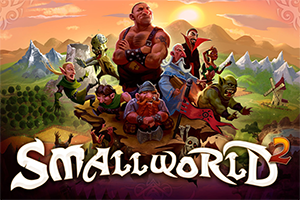
\includegraphics[width=0.8\textwidth]{../../IHM/StartScreen.png}~\\[5cm]
	\end{center}

\newpage
\tableofcontents
\newpage

\section*{Introduction}
Ce jeu est inspiré de SmallWorld. Il s'agit d'un jeu de stratégie à deux joueurs dans lequel chacun dirige un peuple. Les unités des peuples bougent sur les cases de la carte afin de les conquérir, et combattent les unités ennemies. Le but est de contrôler plus de cases que son adversaire.\\

\section{Principes et But du jeu}
	\subsection{Règles du jeu}
		\subsubsection{Peuples}
		Les joueurs ont le choix entre trois peuples : les Orcs, les Elfs et les Nains. Chacun dispose de bonus et malus influant sur la façon de les jouer.

\paragraph{Elfs} Les Elfs ont un coût de déplacement réduit de moitié sur une case Forêt, tandis que le déplacement sur une case Déserte est deux fois plus coûteux. Lors d'un combat dont l'issue conduit à la mort de l'unité, celle-ci a 50\% de chance de s'échapper avec 1 point de vie.
\paragraph{Orcs} Les Orcs ont un coût de déplacement de 50\% sur une case Plaine. Ils ne gagnent aucun point sur une case Forêt, mais ont un bonus propre à l'unité lorsque celle-ci en tue une autre.
\paragraph{Nains} Les Nains ont un coût de déplacement divisé par deux sur une case Plaine. Ils n'acquièrent aucun point sur les cases de ce type. Ils peuvent se déplacer d'une case Montagne à une autre à condition que celle-ci ne soit pas occupée par une unité adverse.

		\subsubsection{Cartes}
		Le joueur, à la création de la partie, a le choix entre trois cartes :
		\begin{itemize}
			\item Small : 2 joueurs, 5 cases x 5 cases, 5 tours, 4 unités par peuple.
			\item Medium : 2 joueurs, 10 cases x 10 cases, 20 tours, 6 unités par peuple.
			\item Large : 2 joueurs, 15 cases x 15 cases, 30 tours, 8 unités par peuple.
		\end{itemize}

		\subsubsection{Déroulement d'une partie}
		Au début du jeu, chaque joueur choisit son peuple. Chaque peuple débute la partie avec toutes ses unités sur la même case de la carte, choisie de manière à ce que les joueurs ne soient pas trop proches. L’ordre de jeu est déterminé aléatoirement en début de partie. Les joueurs jouent chacun leur tour sur le même ordinateur.

	\subsection{Tours de jeu}
	Lorsqu’un joueur peut jouer (c.-à-d. une fois par tour), il peut déplacer toutes ses unités suivant leur nombre de points de déplacement (à part dans le cas d'un bonus lié au peuple, un déplacement sur une case coûte un point de déplacement). Une unité combattante peut engager un combat s’il lui reste au moins un point de mouvement. Une fois le tour terminé, c’est au joueur suivant de commencer son tour. La partie se termine lorsque le nombre de tours prédéfini en début de partie a été effectué, ou lorsqu’il ne reste qu’un seul joueur sur le plateau.

\section{Guide d'utilisation}
	\subsection{Lancement du jeu}
	Pour lancer le jeu, allez dans SmallWorld/IHM et lancez \og IHM.exe \fg{}. Une fenêtre s'ouvre alors dans laquelle vous pouvez choisir de lancer une nouvelle partie ou bien en charger une existante, comme montré sur la Figure \ref{fig:lancement}.
	\begin{figure}[h!]
		\centering
		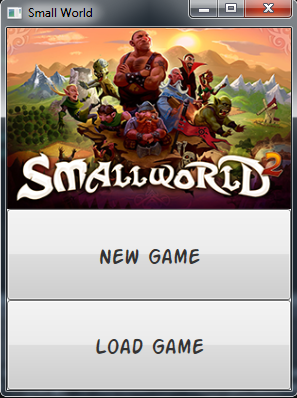
\includegraphics[width=0.4\textwidth]{../../IHM/lancement.png}
		\caption{Fenêtre de lancement du jeu}
		\label{fig:lancement}		
	\end{figure}

		\subsubsection{Nouvelle partie}
		En cliquant sur le bouton \og New Game\fg{} vous pourrez choisir le nom de joueurs ainsi que les peuples que vous désirez jouer. Cette interface est représentée à la Figure \ref{fig:settings}.
		Vous pourrez ensuite lancer la partie en cliquant sur \og Start\fg{}.
		\begin{figure}[h!]
			\centering
			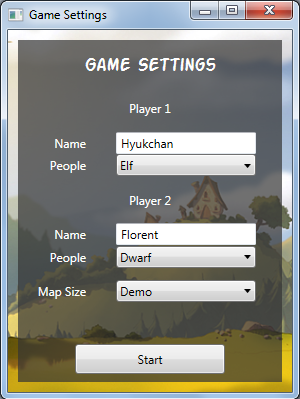
\includegraphics[width=0.4\textwidth]{../../IHM/settings.png}
			\caption{Ecran de configuration de la partie.}
			\label{fig:settings}
		\end{figure}

		\newpage\subsubsection{Chargement d'une partie}
		En cliquant sur le bouton \og Load Game\fg{} vous pourrez choisir la partie à charger. Cet écran est représentée à la Figure \ref{fig:loading}.

	\subsection{Commandes du jeu}
	Une fois la partie lancée, l'écran suivant s'affiche :
		\begin{figure}[h!]
			\centering
			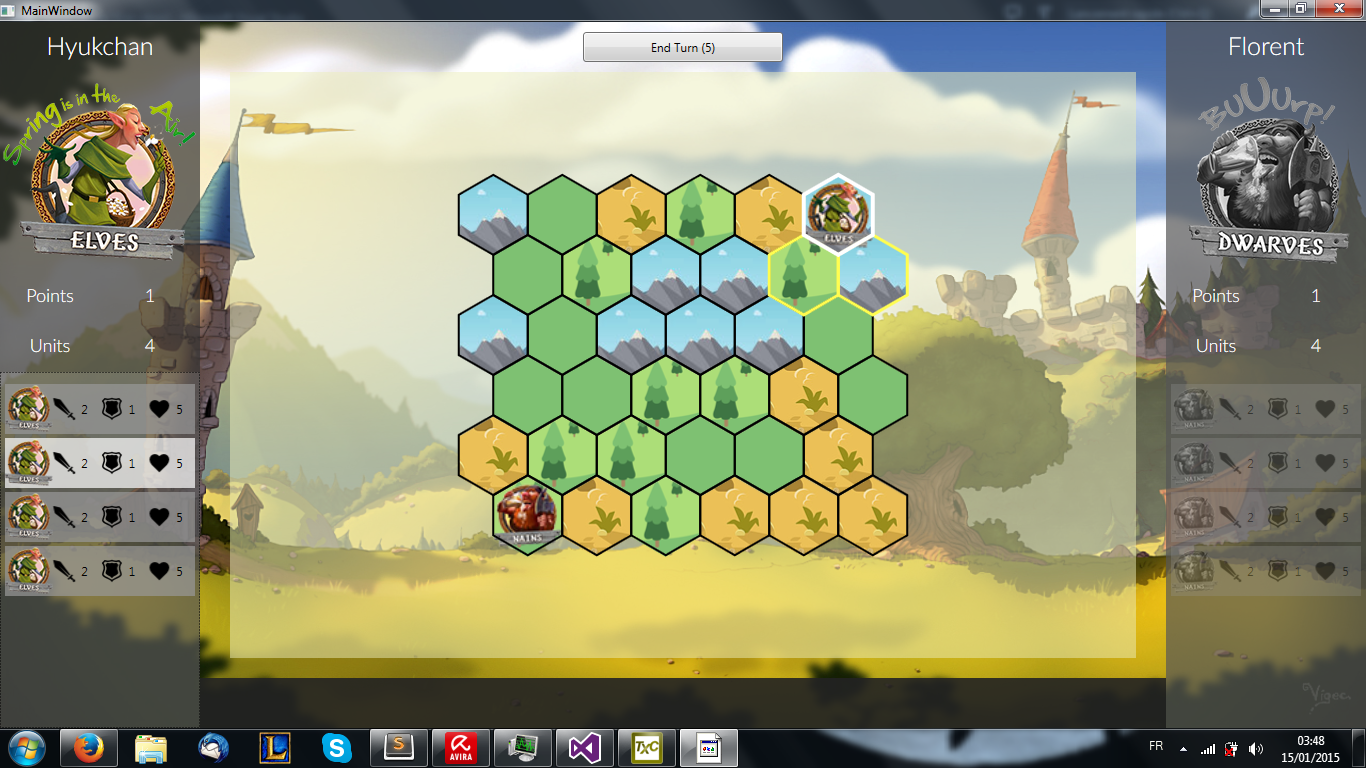
\includegraphics[width=0.9\textwidth]{../../IHM/partie_lancee.png}
			\caption{Partie lancée}
			\label{fig:debut_partie}
		\end{figure}

		Les deux joueurs, leur peuple et leurs unités sont représentés de chaque côté de la fenêtre.
		Le joueur dont le tour est en cours est coloré. Vous pouvez sélectionner une case en effectuant un clic gauche sur une case. Cela sélectionne également les unités présentes sur la case, et les met en valeur. Si plusieurs unités sont présentes sur la case, l'une d'entre elles est sélectionnée au hasard.
		La sélection d'une unité peut également se faire en cliquant sur les unités sur le côté.

		Les déplacements sont possibles après avoir sélectionné une unité. Il faut alors effectuer un clic droit sur la case sur laquelle vous voulez déplacer l'unité.

		Les cases surlignées en jaune représentent des déplacements possibles.




\end{document}